\begin{wrapfigure}[8]{r}{0.48\textwidth}
     \vspace{-5mm}
  \begin{center}
     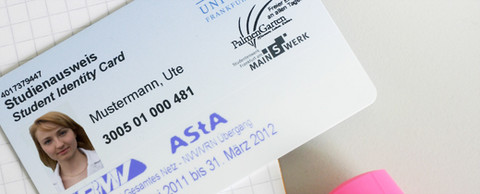
\includegraphics[scale=0.5]{bilder/goethecard}
  \end{center}
\end{wrapfigure}

Nach der erfolgreichen Immatrikulation an unserer Universität bekommst du im Studien-Service-Center eine schicke Chipkarte mit deinem Foto und einigen bildhaften Logos und Beschriftungen drauf. Möglicherweise erfährst du auch gleich, dass sie \emph{Goethe-Card} heißt und als Studienausweis dient. Warum braucht man überhaupt so etwas, wenn man bereits einen ordinären Ausweis hat?

Der wichtigste Grund ist die Tatsache, dass man damit sofort feststellen kann, ob du zum aktuellen Zeitpunkt an der Goethe-Universität studierst: In diesem Fall wurde das blau aufgetragene Gültigkeitsdatum unten zu diesem Zeitpunkt noch nicht überschritten. 

Falls du jetzt einen Blick auf deinen Studienausweis wirfst, wirst du bemerken, dass dort als Enddatum der letzte Tag des laufenden Semesters steht. Daher wirst du, solange du bei uns bleibst, einmal alle 6 Monate diesen Eintrag updaten müssen. Das geht über einen überall auf dem Uni-Gebiet platzierten Automaten, die \emph{Validierer} genannt werden. Sollte man sein Studium erfolgreich beendet oder abgebrochen haben, wird der Validierer das Enddatum der Gültigkeit nicht ändern.

Auf der Goethe-Card sind außerdem dein Foto, dein Name und auch deine persönliche Identifikationsnummer (\emph{Matrikelnummer}) in der Universität aufgedruckt\footnote{Deine Matrikelnummer ist 7-stellig und entspricht den letzten 7 Ziffern der 12\hbox{-}stelligen Zahl auf der Goethe-Card.}. Diese Angaben helfen nicht nur den Profs, dich eindeutig zu identifizieren, sondern auch dir, deine während der Prüfung vergessene Matrikelnummer schnell zu finden.

Aber das ist noch nicht alles, was du mit der Goethe-Card machen kannst:

\begin{itemize}
	\item Du kannst darauf mittels spezieller Geldautomaten-ähnlichen Geräten \textbf{Geld aufladen}, um damit in der Mensa für das Essen oder auch in der Uni-Bibliothek für die Verwendung des Kopierers zu bezahlen.
	\item Du kannst sie als einen \textbf{digitalen Schlüssel} für die super modernen \textbf{Schließfächer} am Campus Westend verwenden
	\item Du kannst damit \textbf{kostenlos} den \textbf{Palmengarten} besuchen.
	\item Du kannst damit \textbf{Bücher} in der \textbf{Uni-Bibliothek} ausleihen.
	\item Du kannst damit \textbf{kostenlos} bestimmte \textbf{Museen} besuchen.
\end{itemize}

Und - last but not least - du kannst damit \textbf{kostenlos} in allen öffentlichen Verkehrsmitteln außer ICE, IC und EC in Hessen und teilweise in angrenzenden Tarifgebieten fahren! 

Das Semesterticket gilt im Gebiet des RMV, NVV, RMV-VRN-Übergangsgebiet und des VGWS. Auf der nächsten Seite findest du eine Karte mit dem skizzierten Geltungsbereich des Semestertickets (Achtung: Stand 2014). Mehr und aktuellere Infos findest du auf den Seiten des AStA Frankfurt:\\
\url{http://www.asta-frankfurt.de/angebote/geltungsbereich-des-semestertickets}.

Au{\ss}erdem: Der Verlust der Goethe-Card kann recht schmerzlich sein - zur Zeit liegt die Gebühr bei Verlust für die Neuausstellung (im Servicecenter des HRZ am Campus Westend) bei 35 Euro. Ist die Goethe-Card defekt bzw. nicht lesbar, kostet euch der Ersatz natürlich nichts.

Man kann mit der Goethe-Card gerade als Informatiker viel Spa{\ss} haben. Der RFID Chip in der Goethe-Card ist sehr gut dokumentiert, einfach auszulesen und zu beschreiben. Suche hierzu Mifare. 

Weitere Informationen zur Goethe-Card kannst du bei Interesse hier finden:\\
\url{http://www.rz.uni-frankfurt.de/44160530/Goethe-Card}

Ach ja, wenn du lieber an der frischen Luft unterwegs bist: Du darfst nach Registrierung auch die /emph{Call a Bike} Leihräder der Deutschen Bahn nutzen. Für die ersten 45 Minuten jeder Fahrt sogar kostenlos (vereinfacht gesagt). Auch hier - mehr Infos beim AStA:\\
\url{http://asta-frankfurt.de/aktuelles/teil-2-wie-leihe-ich-callbike-aus}